\documentclass[10pt,oneside,a4paper,english]{article}
\usepackage[T1]{fontenc}
\usepackage[margin=2cm,headheight=26pt,includeheadfoot]{geometry}
\usepackage[english]{babel}
\usepackage{listings}
\usepackage{color}
\usepackage{titlesec}
\usepackage{titling}
\usepackage[framed, numbered]{matlab-prettifier}
\usepackage{changepage}
\usepackage{amsmath}
\usepackage{hyperref}
\usepackage{cleveref}
\usepackage{enumitem}
\usepackage{subcaption}
\usepackage{graphicx}
\usepackage{fancyhdr}
\usepackage{lastpage}
\usepackage{caption}
\usepackage{tocloft}
\usepackage{setspace}
\usepackage{multirow}
\usepackage{titling}
\usepackage{float}
\usepackage{comment}
\usepackage{booktabs}
\usepackage{indentfirst}
\usepackage{lscape}
\usepackage{booktabs,caption}
\usepackage[flushleft]{threeparttable}
\usepackage[danish]{nomencl}
\usepackage{xcolor}
\usepackage{lipsum}
% \usepackage[backend=biber, sorting=ynt]{biblatex}
% \addbibresource{document.bib}
\usepackage{pdfpages}
\usepackage{amssymb}
\usepackage{bbm}


% \usepackage{relsize}

% --- set footer and header ---
\pagestyle{fancy}
\fancyhf{}

\setlength{\parindent}{0em}
\setlength{\parskip}{10pt}

\title{Active ML and Agency: Miniproject 1} % to reference as \title, dont use \maketitle
\makeatletter\let\Title\@title\makeatother



\lstset{language=Matlab,
style=Matlab-editor,
basicstyle=\normalsize\mlttfamily,
numbers=left,
numberstyle={\scriptsize\color{black}},			% size of the numbers
numbersep=0.5cm											
}

\newlist{steps}{enumerate}{1}
\setlist[steps, 1]{leftmargin=1.5cm,label = Step \arabic*:}
\renewcommand{\headrulewidth}{1pt}
\renewcommand{\footrulewidth}{1pt}

%\lhead{\Title}
\rhead{\nouppercase{\rightmark}}
\lhead{\Title}
\rfoot{
\includegraphics[height=1.25cm]{root/logo.pdf}} % right header logo
\setlength\headheight{16pt}
\setlength{\footskip}{50pt}
\lhead{\Title} %rightH title
\cfoot{\thepage}

% --- End of page settings ---

% Math symbols and operators
\DeclareMathOperator*{\argmax}{argmax} % thin space, limits underneath in displays
\newcommand{\Tau}[0]{\scalebox{1.58}{$\tau$}}
\newcommand{\X}[0]{\mathcal{X}}
\renewcommand{\d}[0]{\text{d}}
\newcommand{\Y}[0]{\mathcal{Y}}
\DeclareMathOperator*{\argmin}{\text{argmin}}
% \newcommand{\Y}[0]{\scalebox{0.85}{$\mathcal{Y}$}}
\newcommand{\ceil}[1]{\lceil {#1} \rceil}
\newcommand{\doubleR}[0]{\mathbb{R}}
\newcommand{\doubleOne}[0]{\mathbbm{1}}
\DeclareMathOperator*{\doubleE}{\mathbb{E}}
\DeclareMathOperator*{\doubleP}{\mathbb{P}}

% begin document

\begin{document}
\pagenumbering{roman} 

\begin{titlepage}
\begin{center}
\vspace{2cm}
%\textsc{ Danmarks Tekniske Universitet}\\[1.5cm]

\includegraphics[width=0.4\textwidth]{root/dtu.png}~\\[1cm]
\vspace{3cm}

% Title
\hrule
\vspace{.5cm}
{ \LARGE \textbf{02466 \\ Project work Bachelor of Artificial Intelligence and Data} \vspace{0.3cm} \\ \LARGE \textit{Conformal Prediction}} % title of the report
\vspace{.5cm}

\hrule
\vspace{1.5cm}

\textsc{\textbf{Authors}}\\
\vspace{.25cm}
\centering

% add your name here
\begin{table}[h]
    \centering
    \begin{tabular}{l c c}
        David Ludvigsen      & s204102 & \texttt{s204102@student.dtu.dk} \\
        Lauge Hermansen      & s204111 & \texttt{s204111@student.dtu.dk} \\
        Torben T. Nguyen & s204121 & \texttt{s204121@student.dtu.dk} \\
    \end{tabular}
\end{table}

\vspace{1.5cm}

% The EMNIST dataset\cite{emnist} has been used to , we use a 

% \vspace{cm}

\end{center}

\begin{center}
    \today % Dags dato
\end{center}
\end{titlepage}


\newpage
\pagenumbering{arabic} 
\fancyfoot[C]{Page \thepage\ of \pageref{EndOfText}}

\section*{Introduction} \label{ch1}


Usually in predictive machine learning, the model returns a point estimate of a target variable, either discrete or continuous, based on some feature variables. However, a lot of the time the model provides no associated uncertainty estimate for its prediction, and in the cases where an uncertainty estimate is provided - these estimates may be dependent upon various assumptions from the model making the uncertainty estimates potentially over/under-confident w.r.t. the validation data. 

In applications where decisions are critical, the transparency of the model's prediction is important for making educated decisions. A calibrated uncertainty estimate adds to this transparency as it enables adaptive attenuation of trust in a model's prediction. This is applicable to many real world implementations of machine learning models. 
\begin{itemize}
    \item In a medical setting, the model may be helping medical professionals with diagnosing patients - a high, calibrated uncertainty for a prediction would function as a warning light to distrust the model.
    \item In a financial setting, the model may be used to price certain services rapidly and automatically - a high, calibrated uncertainty could indicate that human interaction for making a decision is necessary.
    \item In the automobile setting, the model may be used to segment and classify obstructions via the video feeds of a self-driving car - a high, calibrated uncertainty could tell the car to drive more carefully around said obstruction.
\end{itemize}

The aim of this project is to introduce the reader to conformal prediction (CP), which is a mathematical framework for creating calibrated confidence bounds on model predictions. A confidence bound is simply an expansion of a model's point prediction into a prediction set. In the case of classification, the prediction set is merely a set of predicted classes, while in the case of regression, the prediction set is a range of predictions. The size of this prediction set is a calibrated, uncertainty estimate.

%
CP introduces the concept of coverage for the prediction set. It states that on average the probability of the true label being in the prediction set is guaranteed to be greater than or equal to $1-\alpha$, where $\alpha\in]0,1[$ is a hyperparameter. The phrase 'on average' means that it will vary a bit, with different trials, just like the test accuracy of an ML model varies with different training sets. This will be discussed in depth in the theory section.
%Therefore, what is guaranteed to be greater than or equal to $1-\alpha$ is the expectation of the probability that the true label is in the prediction set.
%calibration sets. The calibration set is the partition of the data used to train the conformal predictor, and will be discussed later. The point is that the expectation over calibration sets of the aforementioned probability will be greater than or equal to $1-\alpha$. This is similar to the fact that the test accuracy of a model varies with different training sets.
%
% CP introduces the concept of coverage for the prediction set, which states that the prediction set (on average) has probability will be on average $1 - \alpha$ of including the true label of the target variable, where $\alpha \in ~]0; 1[$ is a hyperparameter.
% The almost magical strength of CP is that applying it guarantees coverage on average.
% %
% %
% Almost even more magical, is that CP is a distribution-free framework and relies upon few assumptions. It is therefore a versatile tool applicable in many different places.
The almost magical strength of CP is that applying it guarantees coverage without distributional assumptions. The only assumption is that the data points are exchangeable. It is therefore a versatile tool applicable in many different places.

The overall aims of the project are as follows:
\begin{itemize}
    \item Investigate and understand the theory behind CP and implement CP with real world data sets and models.
    \item How useful is CP in practice, and how does it compare to other techniques, e.g. Gaussian Process?
    \item Create an extension of CP with transformer networks on sequential data, which violates the exchangability assumption.
\end{itemize}

The general outline of the project is as follows:
\begin{enumerate}
    \item Informal introduction to CP to give an overview of the general ideas.
    \item Mathematical walkthrough of CP to create a rigorous foundation. 
    \item How to do statistical evaluation of implementations of CP to verify correct implementation.
    \item Description and considerations of the dataset used.
    \item Evaluation of CP on a convolutional neural network and logistic regression models.
    \item Comparison of CP vs. gaussian processes.
    \item Extension of CP to work with sequential data while getting around the violation of the exchangability assumption.
\end{enumerate}




\section*{Theory} \label{ch2}
% David doing some explanations
Conformal prediction is an extension to a model used for either a classification or a regression task that include uncertainty measures for the prediction. %The reader can think of CP as a way of reshaping the confidence intervals/sets of the model to statistically rigorous ones. 

The model that CP is applied on needs to output some uncertainty measure, however this measure does not necessarily need to be true or accurate. The goal of CP is to change the uncertainty measure into a statistically rigorous one. 

CP does this in three steps, it defines a score function that maps the uncertainty outputs of the model to some score, then it computes the desired quantile of a calibration set and at last computes the same score on the new data point and selects all scores below this quantile as the prediction set (for regression this last step is slightly different). 

The score function is chosen such that the more certain the model is on the real output the smaller it becomes, hence the further form the truth the models prediction is the larger the score becomes. 

Next the scores are computed for a calibration set and the $\frac{\ceil{(n+1)(1 - \alpha)}}{n}$ quantile is chosen as $\hat{q}$. This choice will be explained later, but the reader can think of this as the desired $1 - \alpha$ quantile when $n$ is large. 

At last, the score function of each label is computed for the new data point. All labels with scores below $\hat{q}$ are in the prediction set. 

With these three steps CP ensures coverage of the prediction set. This coverage means that $1 - \alpha$ amount of the time when this entire procedure is performed the true label is in the prediction set for one new sample. This does not mean that $1 - \alpha$ amount of label predictions done with one realization of the algorithm will contain the true label. To get an intuition for this the reader can imagine being unlucky with the calibration set such that the calibration set does not represent the underlying distribution accurately. Hence, the confidence intervals will be quite poor. However, this will only happen rarely. As will be explained later the accuracies of each realization of a calibration set will be beta distributed with an expectation of $1 - \alpha$. 

Next the algorithm will be explained mathematically. 
% notations and definitions
\subsection*{Notation and definitions}
Conformal Prediction is a way of doing uncertainty quantification without distributional assumptions or model assumptions. The only assumption is that all data points are exchangeable.\\
%
The goal of CP is to create valid confidence bounds from an existing model. Mathematically formulated the aim is to create a function, $\Tau: \X \rightarrow T$, that maps a data point from the input space to a subset of the output space, such that
\begin{gather}
\doubleP(y\in\Tau(X)) \geq 1-\alpha, \quad \forall X\in\X.
\label{eq: coverage}
\end{gather}
Here, $X$ is a sample, $y$ is its corresponding true label, $\X$ is the input space, $\Y$ is the space of the target value, and $T = \{t:t\subseteq \Y\}$ are all possible subsets of $\Y$. In the future we will refer to elements in $T$ as either prediction sets or prediction intervals depending on the task; classification or regression respectively. Finally $\alpha$ is a pre-specified error rate, i.e. the chance of the true label being outside the prediction set.
% Description of the method - The algorithm
\subsection*{Description of the method}
\label{sec: description of method}
First a machine learning (ML) model,
$f: \X\rightarrow \Y$,
suitable for the given task is chosen.
Then a score function,
$s:\X\times\Y\rightarrow\doubleR$,
is specified.
The score function is a heuristic, but in order for CP to be useful it should grow with the difficulty of the input. Once the score function is chosen, split the data into 3 splits: A training set, $(X^{train}, y^{train})$, a calibration set, $(X^{cal}, y^{cal})$, and a validation set, $(X^{val}, y^{val})$. The training set is used to train the underlying ML model, $f$, e.g. a neural network.

The calibration set is used to train, or 'calibrate', the conformal predictor. It does so by computing the scores, $s_i = (X^{cal}_i, y^{cal}_i)$ for each data point in the calibration set. Here $(X^{cal}_i, y^{cal}_i)$ is the $i^{th}$ calibration point and its corresponding true label. Then let $\hat q$ be the $\ceil{(1-\alpha)(n+1)}/n$ quantile of the scores in the calibration set. Finally, $\Tau$ is defined such that 
\begin{gather}
\Tau(X) = \{y\in\Y : s(X,y) \leq \hat q\},
\label{eq: def. prediction set}
\end{gather}
where $X\in\X$ is one data point. In words, $\Tau(X)$ returns the possible $y\in\Y$ such that the score function of $(X,y)$ is less than or equal to $\hat q$. Note that $\hat q$ is an estimate of the true $1-\alpha$ quantile of the score distribution. Finally, the validation set is used to validate that \cref{eq: coverage} holds by estimating expectation below
\begin{gather}
    \doubleP(y\in\Tau(X)) = \doubleE\left[\doubleOne\left(y\in\Tau(X)\right)\right] \approx \frac{1}{n_{val}}\sum_{i=1}^{n_{val}}\left[\doubleOne\left(y^{val}_i\in\Tau(X^{val}_i)\right)\right]
    \label{eq: coverage expactation}
\end{gather}

% 
% Exchangeability 
%
\subsection*{Exchangeability}
CP requires very few assumptions unlike many other probabilistic models. It requires that the data samples in the calibration and validation set are exchangeable. Here it is important to explain the distinction between exchangeable and i.i.d. data points. Exchangeable means that 
\[
P_{X, Y}(X=x, Y=y) = P_{X, Y}(X=y, Y=x)
\]
which might seem the same as i.i.d. as we state that x and y need to follow the same distribution. However, exchangeability allows $X$ and $Y$ to be correlated because of a shared confounder. This also means that conditionally on all confounders, exchangeable random variables are independent.
\[
P_{X, Y}(X=x, Y=y|Z=z) = P_{X, Y}(X=y, Y=x|Z=z) = P_{X}(X=y|Z=z)P_{Y}(Y=x|Z=z)
\]
Here $Z$ describes all confounders for $X$ and $Y$ and they are therefore conditionally independent. 
%
% Proof of coverage.
%
\subsection*{Proof of coverage}
Now follows the proof that the statement in \cref{eq: coverage} is actually true when applying CP. Let $s_i$ be the score function of the $i$'th data point in the calibration set, i.e., $s_i=s(X_i^{cal},y_i^{cal})$ for $i=1,2,\dots,n$, where $n$ is the number of data points in the calibration set. These will be referred to as calibration scores.
Now, let $s'$ be the score of a new data point, $X$, with true label, $y$. Since the scores are assumed exchangeable, the probability that the rank of $s'$ is at most $k$ is $k/(n+1)$. Here $rank(s')=k$ means that $s'$ is the $k$'th smallest element in the set. This is because the calibration scores together with $s'$ are $n+1$ exchangeable random variables, so the chance of either one of them having a specific rank for any realization is exactly $1/(n+1)$. As there are $k$ different ranks less than or equal to $k$, this yields
\begin{gather}
    \doubleP(rank(s')\leq k) = \frac{k}{n+1}
    \label{eq: prob k}
\end{gather}
% \begin{gather}
%     \doubleP(s'\leq s_k) = \frac{k}{n+1}
%     \label{eq: prob k}
% \end{gather}
% where the scores have been reordered such that $rank(s_k)=k$.\\
Due to the construction of $\Tau$, $y$ is in the prediction set of a data point $X$, if and only if the score function of $(X,y)$ is less than or equal to $\hat q$, i.e., 
\begin{gather*}
    y\in\Tau(X) \Leftrightarrow s' \leq \hat q
\end{gather*}
This means that
\begin{gather}
    \doubleP(y\in\Tau(X)) = \doubleP(s' \leq \hat q)
    \label{eq: pred set prob}
\end{gather}
By definition, $\hat q$ is the value of the calibration score with rank $\ceil{(n+1)(1-\alpha)}$. Therefore, making the substitution $k := \ceil{(n+1)(1-\alpha)}$ in \cref{eq: prob k}, has the result
\begin{gather*}
    \doubleP(s'\leq \hat q)
    = \doubleP\big(rank(s') \leq \ceil{(n+1)(1-\alpha)}\big)
    = \frac{\ceil{(n+1)(1-\alpha)}}{n+1}
    \geq \frac{(n+1)(1-\alpha)}{n+1}
    = 1-\alpha
\end{gather*}
Finally, combining this with \cref{eq: pred set prob}, we arrive at
\begin{gather}
    \doubleP(y\in\Tau(X)) \geq 1-\alpha
\end{gather}
The goal is to prove an upper bound of coverage as well, as it exists, but we haven't gotten that far yet.
%
%
%
%
%
%
%
%
\subsection*{Statistical evaluation of coverage}
The coverage will now be examined. First, let $C$ be the estimated coverage, and let $\mu$ be the true coverage as defined in \cref{eq: coverage expactation}.
%
\begin{gather}
\label{eq: coverage mu}
C = \frac{1}{n_{val}}\sum_{i=1}^{n_{val}}\left[\doubleOne\left(y^{val}_i\in\Tau(X^{val}_i)\right)\right]\\
\label{eq: coverage C}
\mu = \doubleE_{\X \times\Y}\left[\doubleOne\left(y\in\Tau(X)\right)\right]=\doubleE[C]
\end{gather}
%
The notation in the definition of $\mu$ means that it is an expectation over the entire input and output space. However, the function $\Tau$ depends on the calibration set, so for different calibration sets, the expectation, $\mu$, will have different values. Hence, the expectation is a random variable itself. This aligns well with the intuition that $\hat q$ is only an estimate of the true $1-\alpha$ quantile of the scores, so different calibration sets will have different coverage. One could imagine an unlucky realization of a calibration set that would yield a coverage lower than $1-\alpha$. However, this seems to contradict the fact that the lower bound of coverage was just proven to be $1-\alpha$.

The key is to look at \cref{eq: prob k}. It only holds because all the $s_i$'s and $s'$ are $n+1$ random variables that are realized simultaneously. If instead the $s_i$'s were already realized, the equality in \cref{eq: prob k} would not hold, because naturally, the probability of $s'$ having rank $k$ would depend on the realizations. Specifically, assuming the $s_i$'s are in sorted order, the probability is given by,
\begin{gather}
    \doubleP\left(rank(s')\leq k\right) =
    P_S(s_k) = \int_{-\infty}^{s_{k}} p_S(s) \d s ,
\end{gather}
where $p_S$ is the probability density function for the scores, $P_s$ is its cdf, and $s_k$ is the $k$'th largest element of the realizations. Assume again that the $s_i$'s are random variables. These reflections show that, the coverage guarantee only holds for each conduction of the procedure - not for a specific realization of calibration set. Equivalently, the proof guarantees that the expectation of $\mu$ is greater than or equal to $1-\alpha$, but not every realization of $\mu$.

In fact, $\mu$ is a probability, and as usual with probabilities of probabilities, $\mu$ follows a beta distribution. Turning the attention to $C$ it appears to be a sum of indicator variables, so it is tempting to conclude that $C\cdot n_{val}$ follows a binomial distribution with parameters $(n_{val}, \mu)$. This is true when conditioning on a calibration set, because then $\mu$ is fixed. However, since $\mu$ follows a beta distribution, $C\cdot n_{val}$ actually follows what's called a BetaBinomial distribution. To sum up,

\begin{gather}
    C|\mu \sim \frac 1{n_{val}} Binom\big(n_{val},\mu\big),
    \quad \text{where} \quad
    \mu \sim Beta(a, b)
\end{gather}
which means that,
\begin{gather}
    C \sim \frac 1{n_{val}} BetaBinom(n_{val}, a, b)
\end{gather}

where $a = \ceil{(n+1)(1-\alpha)}$ and $b=\lfloor(n+1)\alpha\rfloor$.
% In a future version of the report, the proof that $\mu$ follows a beta distribution will be featured here.
%Now follows a short elaboration on why the parameters to the beta distribution make sense. In a beta distribution the parameters $a$ and $b$ can be thought of as the number of successes and failures respectively, and here we define a success as the true label being in the prediction set. Recall that the calibration set size is $n$ and $\hat q$ is defined as the $a$'th element in the calibration scores. Then it makes sense to say that the prior knowledge of $\mu$ is $a$ successes and $b$ failures, because in fact
% \begin{gather}
%     a+b=\ceil{(n+1)(1-\alpha)}
%     + \lfloor(n+1) \alpha\rfloor = n+1,
% \end{gather}
% and we had exactly $n+1$ elements in the proof.

\subsubsection*{Proof of coverage following a beta distribution}
Now follows the proof that $\mu$ follows a beta distribution. For that, turn the attention to \cref{eq: pred set prob}. For a given realization,
\begin{gather*}
    \doubleP(s'\leq \hat q) = P_S(\hat q),
\end{gather*}
and therefore,
\begin{gather*}
    \mu = \doubleP(y\in\Tau(X)) = P_S(\hat q),
\end{gather*}
where $P_S$ is the (unknown) cdf for the scores.

This means that $\hat q$ tries to estimate the true $1-\alpha$ quantile, but actually it is the $\mu$ quantile. Therefore, the goal is to find a pdf, $f$, for $\mu$.

Let $S_i,~for~ i=1,2,\dots,n$ be exchangeable random variables representing the permutation that sorts the scores of the $n$ data points in the calibration set. To understand this, recall the example with the rocks. We will just extend the example to having $n$ spots where we will put the rocks We know we will collect $n$ scores, and $S_i$ will represent a spot that is reserved for the $i$'th smallest score. Furthermore let $U_i = P_S(S_i)$, that is, $U_i$ is the random variable that represents the mapping the $i$'th score to the true quantile. Due to the definition of $P_S$, $U_i$ follows a uniform distribution. For each realization, i.e. calibration set, the probability of $\mu$ being in a specified range, $[m, m+\delta m]$, is the probability of either $U_i$ having rank $a$ \textit{and} being in that range. For easier overview we choose $i=a$, but that is an arbitrary choice. That is,
\begin{align}
    \doubleP(\mu \in [m,m+\delta m])
    \nonumber
    &= \doubleP\big(U_a \in [m,m+\delta m] , rank(U_a) = a\big)\\
    &= \doubleP\big(U_a \in [m,m+\delta m]\big)\cdot \doubleP\big(rank(U_a) = a\big)
    \label{eq: prob mu in range}
\end{align}
Note that since $U_i$ is uniform
\begin{gather}
    \doubleP\big(U_a \in [m,m+\delta m]\big) = \delta m
    \label{eq: prob Ua in range}\\
    \nonumber
    \doubleP\big(U_i < m\big) = m\\
    \nonumber
    \doubleP\big(U_i > m + \delta m\big) = 1-m-\delta m
\end{gather}
Also note that $a+b=n+1$, and  $\Gamma(x) = (x-1)!,~ \forall(x\in\mathbb{N})$ so,
\begin{align}
    \nonumber
    \doubleP\big(rank(U_a) = a\big)
    &= \doubleP\big(U_{1,2,...,a-1} < m , ~U_{a+1,a+2,...,n} > m+\delta m\big)\\
    \nonumber
    &= m^{a-1}\begin{pmatrix}n\\a-1\end{pmatrix}    \cdot (1-m-\delta m)^{n-a} \begin{pmatrix}n-a+1\\n-a\end{pmatrix}\\
    \nonumber
    &= m^{a-1} \frac{(a+b-1)!}{(a-1)!b!}\cdot (1-m-\delta m)^{b-1}b\\
    &= m^{a-1} \frac{(a+b-1)!}{(a-1)!(b-1)!}\cdot (1-m-\delta m)^{b-1}
    \label{eq: prob rank Ua = a}
\end{align}
The notation $\doubleP\big(U_{1,2,...,a-1} < m)$ is shorthand for $\doubleP\big(U_1 < m, U_2 < m, ... , U_{a-1} < m)$.

Pluggin \cref{eq: prob rank Ua = a} and \cref{eq: prob Ua in range} into \cref{eq: prob mu in range}, and combining with the definition of probability density, we arrive at
\begin{align}
    f(m) &= \lim_{\delta m \rightarrow 0} \frac{\doubleP\big(\mu\in[m,m+\delta m]\big)}{\delta m}\\
    &= \lim_{\delta m \rightarrow 0} m^{a-1} \frac{(a+b-1)!}{(a-1)!(b-1)!}\cdot (1-m-\delta m)^{b-1}\delta m \frac{1}{\delta m}\\
    &= m^{a-1}(1-m)^{b-1}\frac{\Gamma(a+b)}{\Gamma(a)\Gamma(b)}
\end{align}
which is exactly the beta distribution with parameters $a = \ceil{(n+1)(1-\alpha)}$ and $b=\lfloor(n+1)\alpha\rfloor$.
%
% Marginal vs. Conditional coverage 
%
\subsection*{Coverage - marginal vs. conditional}
Coverage in itself is not impressive as a model with $100\%$ coverage can easily be made by returning the entire output/label space for each data point. This is not useful at all and it is therefore preferable to obtain coverage with the smallest prediction set possible (this will however depend a lot on the model because if that is not well suited for the task the prediction set from CP will be large). 

Next we distinguish between marginal coverage and conditional coverage. Marginal coverage entails that the procedure will classify a new data sample correctly $1 - \alpha$ amount of the time, however, it might not classify all groups equally well. An example could be a prediction task with where the model needs to find out if a patient has a disease or not. This disease is quite rare and only one out a hundred has it. This means that a model that just classifies all patients as not having the disease will obtain marginal coverage of $99\%$. 

A more useful property is conditional coverage which state that the model will obtain coverage within each group. In the previous example the model would need to at least correctly classify $1-\alpha$ of the sick people as sick and $1 - \alpha$ of healthy people as healthy.

In the future, we will feature metrics for conditional coverage.

\section*{Data} \label{ch3}
A real problem setting is investigated to evaluate how CP is affected by different factors such as which type of model is used for the predictions. As any model can be extended with CP, the problem setting and the model will be sculptured from a previous paper; \textit{"Active Machine Learning and Agency - Bayesian Optimization on EMNIST"}. 

In this paper the EMNIST data set is used, which contains images of grey scaled hand written numbers and letters in a $28 \times 28$ resolution. The data set distinguishes cases of the same letter which yields $62$ different classes. The training set contains $697,932$ data point split equally among the $62$ classes, but only $279,173$ ($40\%$) stratified data points are used for the training of the model. The test set contains $116,323$ data point, but only batches of $500$ are used as calibration sets.  

Below the six random data points are drawn to get an idea of how the data set looks. 

\begin{figure}[H]
    \centering
    
\includegraphics[width=0.85\textwidth]{Images/letters_clipped.png}
    \caption{Six hand written letters and numbers.}
    \label{fig:cnn_architecture}
\end{figure}

In this project the data set is only used to evaluate CP and the contents of the data set is therefore not important. However, when deploying CP one must evaluate the data set. An example is given with this data set. The EMNIST data set is written by 500 different writers and was collected in 1995. This might create some kind of bias only letters from these 500 people were sampled. An even more important potential bias is that there could be a cultural difference between the 500 authors and the group this letter/number recognizer is supposed to classify. 

Although CP upholds coverage this will not mean that the biases in the dataset will be eradicated. If the data set contains some sort of inherent bias the conformal predictor will too. However, if the calibration set does not, our conformal predictor won’t either. This is important in real world settings where the model might be trained on a biased data set (only US citerzins with a specific pencil write the letters), but is then applied to the data it is going to be used for. While the model is in use, a calibration set can slowly be gathered from the data that does not include a bias and the conformal predictor model can be deployed without a the bias! This does not mean that the model will somehow learn and erase this bias from its previous learning, but instead that the confidence sets will become larger and uphold coverage. 
\section*{Methods} \label{ch4}
The guarantees of CP can be applied to many different types of models. Different models, however, predict differently which may influence coverage and the prediction sets in practice. This influence may be significantly quantifiable.

CP can be extended by TODO TODO TODO. The performance is compared to TODO TODO TODO TODO

We will figure the TODO's out later

% 

\subsection{Behavior under different models}
Different model types trained on the same training data may have different prediction sets after application of CP and testing. The prediction sets can differ in both content and size, however, this difference may in practice be insignificant. This project will examine whether the prediction set size is significantly different between a convolutional neural network vs. a multinomial logistic regression model on a classification task on the EMNIST dataset.


\subsubsection{Models}
The logistic regression model is trained on the standardized, flattened feature vectors of each image. The model is implemented using the scikit learn logistic regression class with default arguments. The model therefore makes use of L2 regularization with a strength of $1$.

The trained convolutional neural network from \textit{Active Machine Learning and Agency - Bayesian Optimization on EMNIST} is reused. The CNN has $4$ convolution layers with a $3$×$3$
kernel, ReLU activation function; $4$ Max-pooling layers with a $2$×$2$ kernel. At the convolutional layer $i$, we set the number of feature maps to be $4 \cdot 2^i$. At the first convolutional layer, we then output $8$ feature maps. As the output layer, we have a single feed-forward layer before our output. The network was trained for $2$ epochs using a batch size of $200$ with a learning rate of $10^{-3}$ and a weight decay of $10^{-5}$. 

\begin{figure}
    \centering
    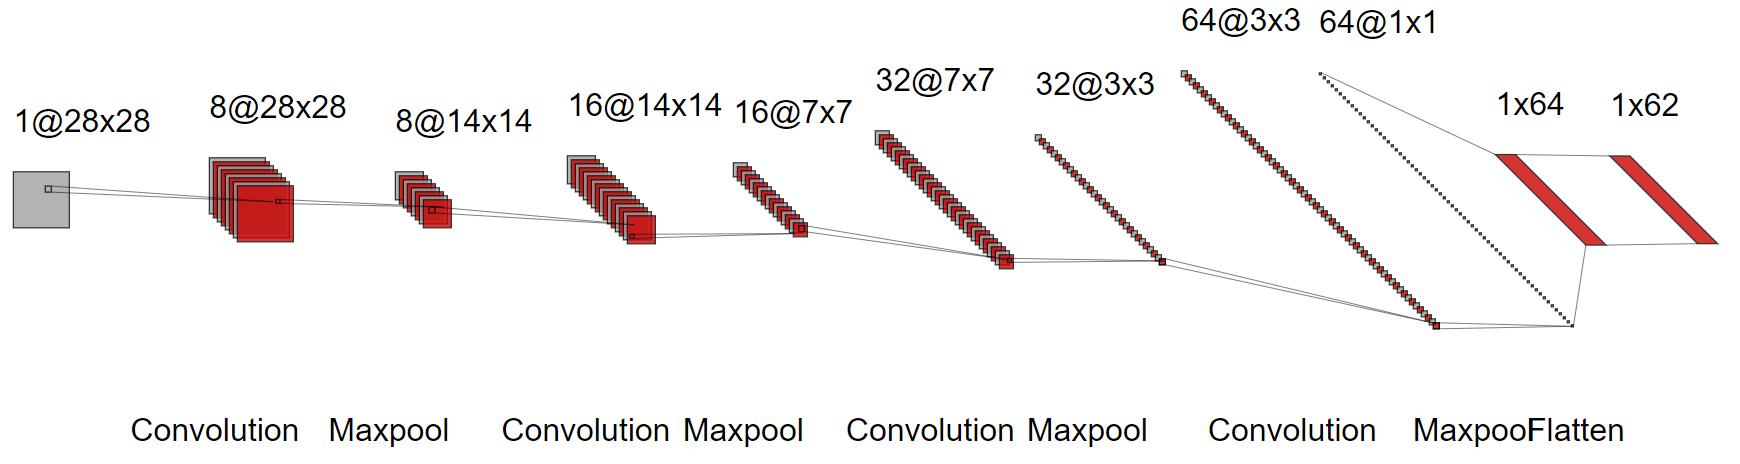
\includegraphics[width=0.8\textwidth]{Images/CNN_arch.png}
    \caption{Architecture of the convolutional neural network model}
\end{figure}


\subsubsection{Adaptive Conformal Prediction}
% The output probabilities of each model then have a conformal prediction framework applied on top. In this case a CP method called Adaptive Prediction Sets. The short description of this CP method is that it figures out how much of the output probability mass on average, $\hat{q}$, must be contained in the prediction set to gain coverage, and then it simply adds the classes with the highest probability mass to the prediction set until the required amount of probability mass has been obtained.
%
One framework for applying CP used in this report is called adaptive prediction sets. It is applicable for classification tasks, where the model outputs a probability distribution over the output classes, such as an ANN with softmax output or multinomial logistic regression.
The score function is then the cumulative sum of the probabilities in decreasing sorted order. That is, if $f_y(X)$ denotes the model output of the data point $X$ corresponding to the class $y$, then the score function is given by,
%
\begin{gather}
    s(X,y)=\sum_{i = 1}^k f_{\pi_i}(X), \quad \text{where $y = \pi_k$ and }k = \argmin_{i} [f_{\pi_i(X)} = f_y(X)]
\end{gather}
Here, $\pi_i$ is the class corresponding to the $i$'th largest model output. In case of ties, the last equality that defines $k$ means that we choose $k$ as small as possible.
% \begin{gather}
%     s(X,y)=\sum_{c\text{ :} f_c(X)\geq f_y(X)}f_c(X)
% \end{gather}
%
% Define $f_c(x)$ as the model's output probability for class $c$ on an image $x$. In addition, also define $f_{(-i)}(x)$ as the model's $i$'th highest output probability on an image $x$. Pay special attention to the parenthesis around $-i$, which denotes that it is an order statistic. The associated class for the second highest output probability would be $c_{(-2)}$. The score function is then given as:
% \begin{align*}
%     s(x, y) = \sum^{k}_{i=1} f_{c_{(-i)}}(x)
% \end{align*}
% Where $y$ is the class label for image $x$, and $k$ is given by $y = c_{(-k)}$.
%

In other words, sort all the output probabilities in descending order, and then sum them until the correct class is reached. This gives the score
% , $s$, for a prediction 
and it represents how much probability mass was required for the correct class to be included in the prediction set.
%
Then a procedure similar to the one described in the methods section is performed with $\hat q$ being the $\ceil{(n+1)(1-\alpha)}/n$ quantile of the calibration scores.
%and the prediction set defined as in \cref{eq: def. prediction set}
% The score is then calculated for the whole calibration set, and the quantile, $\hat{q}$, for some $\alpha$ is found as previously described. This quantile represents the amount of probability mass to include to gain marginal coverage. 

After the $\hat{q}$ has been found, a prediction set can be constructed as follows:
\begin{align*}
    \Tau(X) = \left\{ \pi_i, \ldots, \pi_k \right\}, ~\text{where}~ k = \text{inf}~ \left\{k' : \sum^{k'}_{i=1} f_{\pi_i}(X) \geq \hat{q} \right\}
\end{align*}
The equation says to include all the $k$ classes with the highest probability mass, such that the sum of the $k$ probability masses is above or equal to $\hat{q}$. The smallest possible $k$ where that is true is used.


\begin{figure}
    \centering
    \begin{subfigure}{0.44\textwidth}
        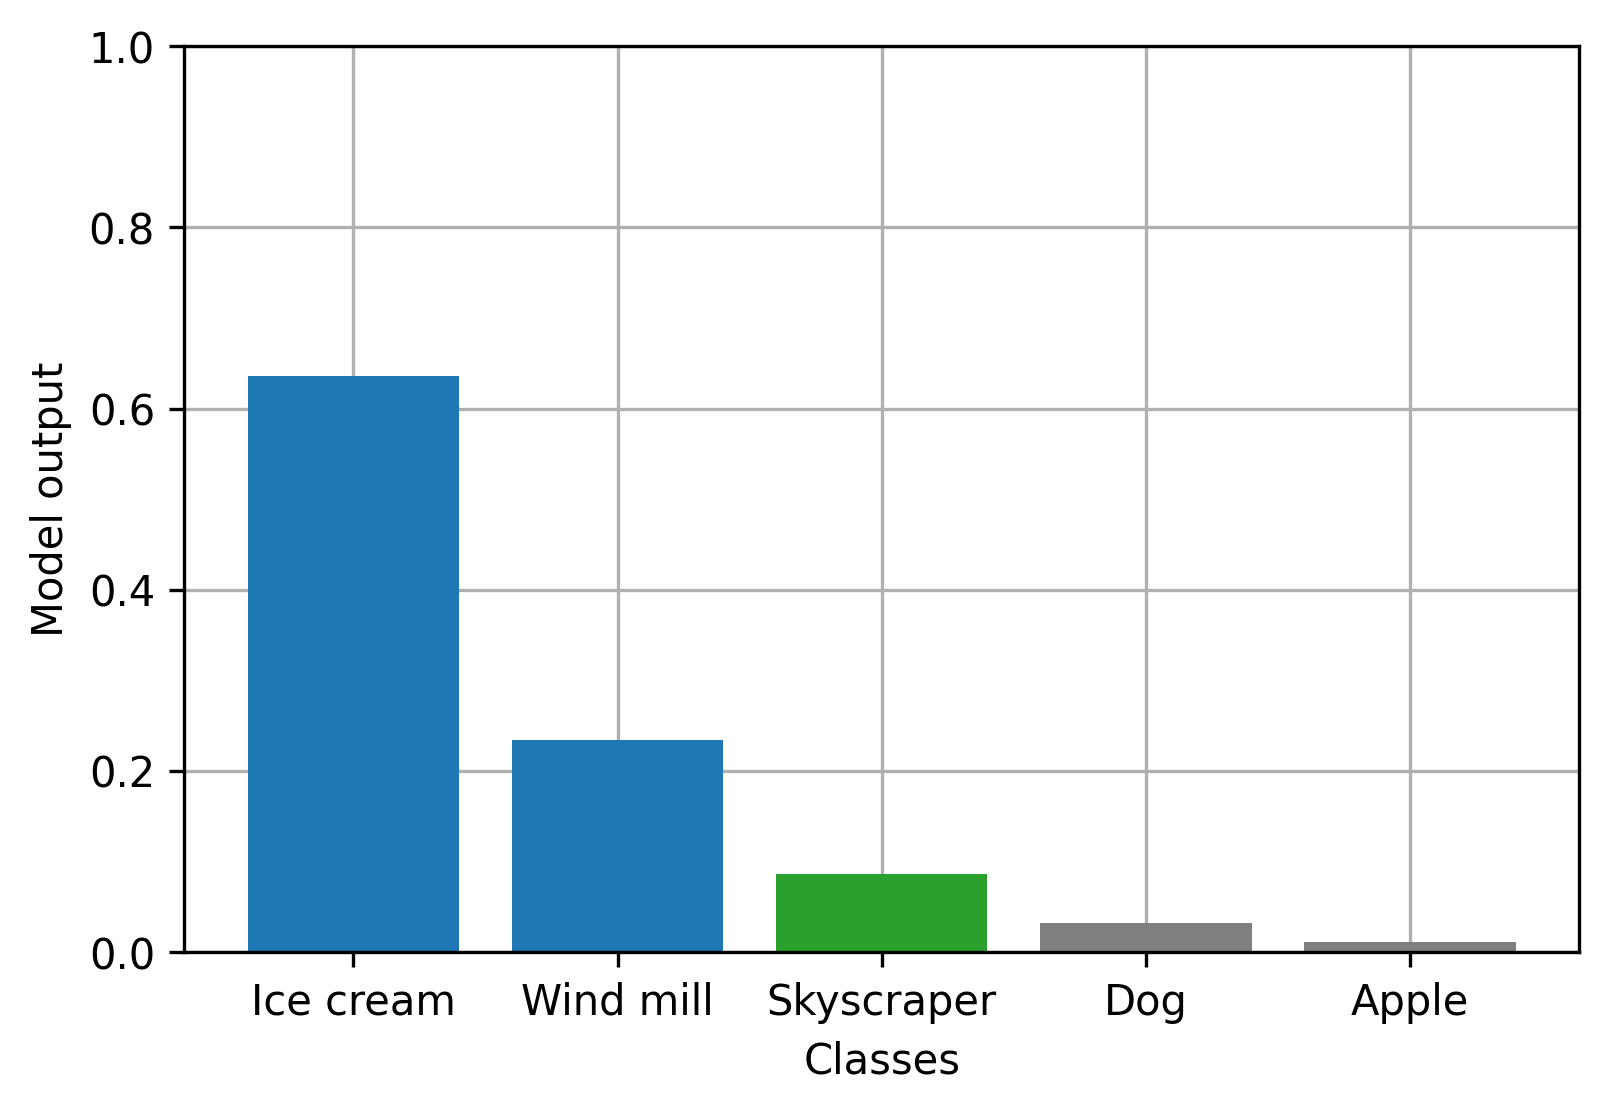
\includegraphics[width=\textwidth]{Images/adaptive-prediction-sets-score.png}
        \caption{Sorted model output for one image. The green class is the label for the image. The score is calculated as the sum of the probabilities of the blue and green classes.}
    \end{subfigure}
    \hspace{1em}
    \begin{subfigure}{0.44\textwidth}
        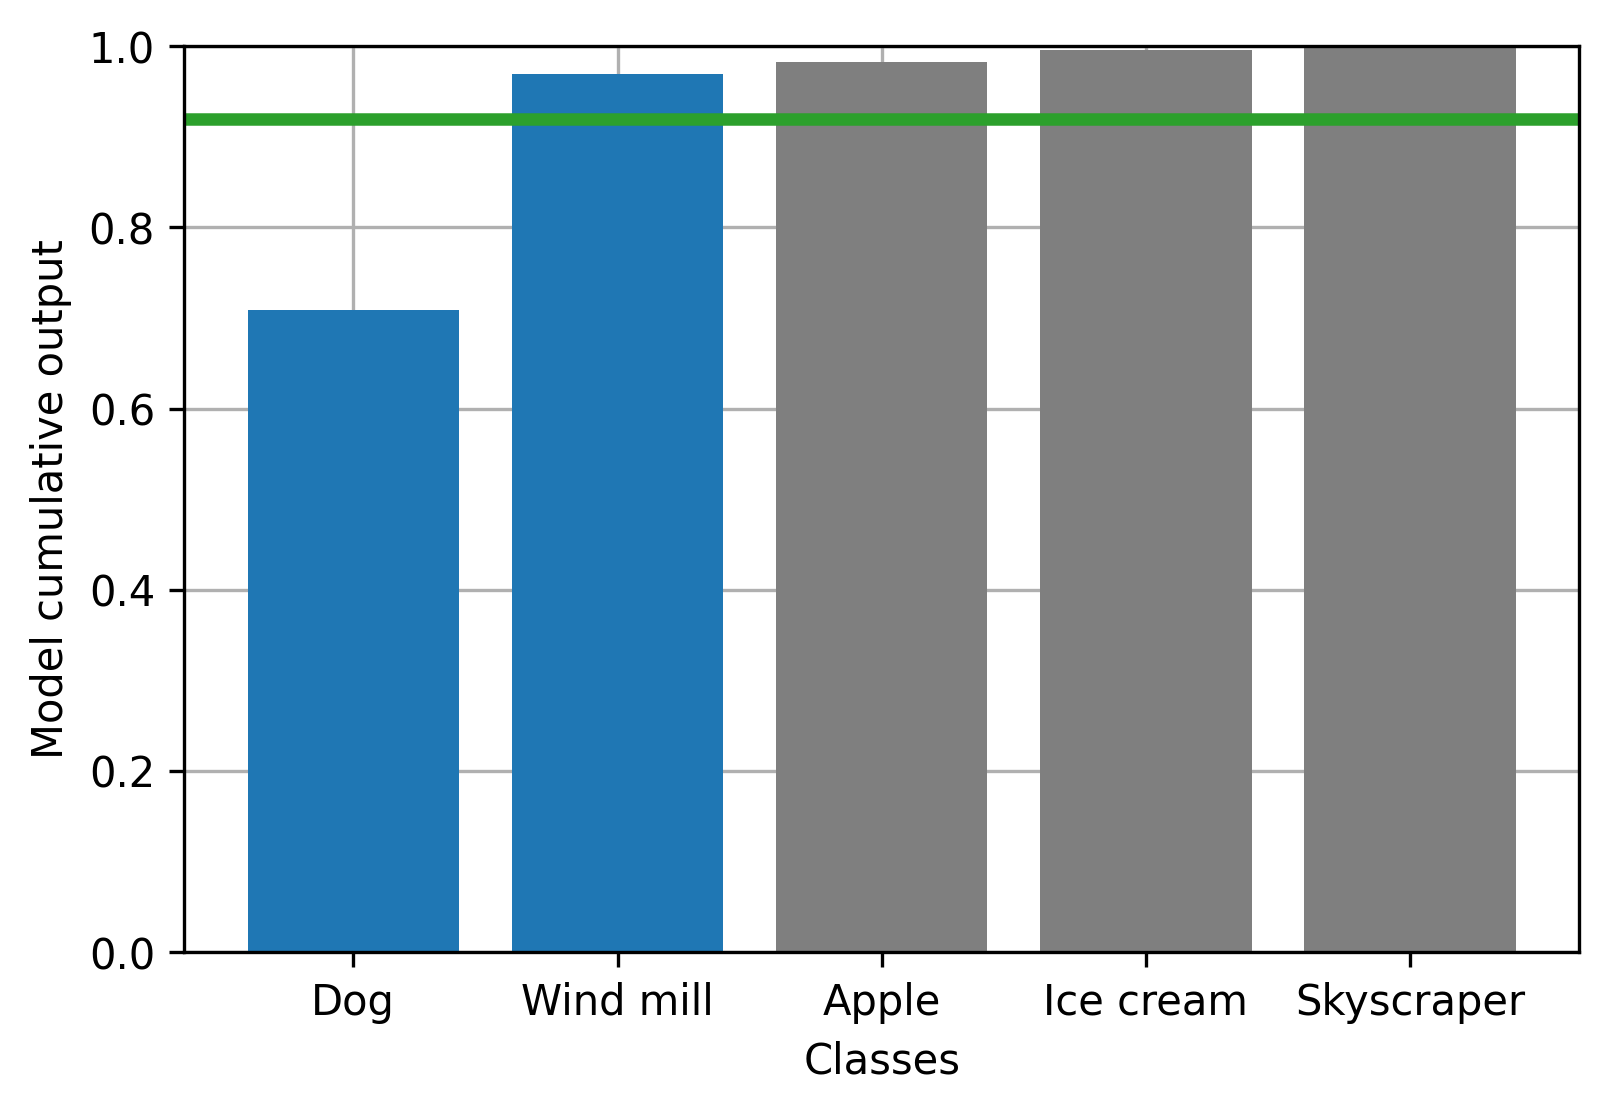
\includegraphics[width=\textwidth]{Images/adaptive-prediction-sets-prediction.png}
        \caption{Cumulative probability mass of sorted model output. The green line represents the quantile $\hat{q}$, while the blue classes represent the prediction set.}
    \end{subfigure}

    \caption{Visual example of calculations for Adaptive Prediction Sets. Note that the two figures come from different data points}
\end{figure}


\subsubsection{Evaluation}
A model with higher accuracy should naturally have smaller prediction sets on average with adaptive CP. Models with equivalent accuracy may, however, still differ in their prediction set sizes in that the distribution of the prediction set sizes may vary. 

Both models are trained on the same training data, calibrated on the same calibration data, and tested on the same test data. The prediction set size for each model for each test point is stored. Analysis is run on these pairs of prediction set sizes.

The prediction set size empirical densities are first plotted for each model and qualitatively evaluated. If the densities seem approximately normal and their variances seem approximately homogeneous, a paired t-test is used. The difference in prediction set sizes for test images is tested against the hypothesis of said difference being zero. If the densities appear to not be normally be distributed or have inhomogeneous variance - a Wilcoxon paired difference test is used in place of the paired t-test. If it turns out that no difference can be detected, a Kolmogorov-Smirnov test can in addition to a qualitative evaluation of the empirical densities be used to discuss the shape of the distribution.


\subsection{Extension of CP}
To be decided. Unable to write about for now.
\label{EndOfText}

\newpage
\pagenumbering{Roman} 
\fancyfoot[C]{Page \thepage\ of I}
\rhead{References}
% \bibliographystyle{ieeetr}
% \printbibliography
\label{endOfDoc}
\end{document}
